\documentclass[11pt,a4paper]{article}
\usepackage[margin=21mm]{geometry}
\usepackage[T1]{fontenc}
\usepackage{lmodern,amsmath,amssymb,booktabs,graphicx,microtype}
\usepackage[colorlinks=true,allcolors=blue]{hyperref}
\usepackage[font=small,labelfont=bf]{caption}
\setlength{\parindent}{0pt}
\setlength{\parskip}{5pt}
\newcommand{\Critical}{1.56489264}
\newcommand{\OrderL}{1.9676}
\newcommand{\OrderH}{0.9957}
\newcommand{\PenaltyOrder}{0.8599}
\newcommand{\FineL}{1.328\times10^{-3}}
\newcommand{\FineH}{1.090\times10^{-1}}
\newcommand{\PatchN}{8.882\times10^{-16}}
\newcommand{\PatchP}{2.682\times10^{-2}}
\newcommand{\Residual}{1.709\times10^{-16}}
\newcommand{\CoarseL}{1.957\times10^{-2}}
\newcommand{\NearL}{3.314\times10^{-1}}
\newcommand{\NearCondition}{2.082\times10^{3}}
\newcommand{\HighCondition}{3.284\times10^{5}}
\newcommand{\QuadLoad}{3.025\times10^{-13}}
\newcommand{\QuadSolve}{1.390\times10^{-13}}
\newcommand{\QuadNorm}{7.772\times10^{-16}}
\newcommand{\ConvergenceRows}{Penalty & 4 & $5.298\times10^{-2}$ & $7.848\times10^{-1}$ & $1.374\times10^{-1}$ \\
Nitsche & 4 & $6.495\times10^{-2}$ & $8.021\times10^{-1}$ & $5.473\times10^{-2}$ \\
Penalty & 8 & $2.372\times10^{-2}$ & $4.248\times10^{-1}$ & $6.737\times10^{-2}$ \\
Nitsche & 8 & $1.957\times10^{-2}$ & $4.284\times10^{-1}$ & $1.327\times10^{-2}$ \\
Penalty & 16 & $1.316\times10^{-2}$ & $2.189\times10^{-1}$ & $3.369\times10^{-2}$ \\
Nitsche & 16 & $5.194\times10^{-3}$ & $2.173\times10^{-1}$ & $3.179\times10^{-3}$ \\
Penalty & 32 & $7.253\times10^{-3}$ & $1.110\times10^{-1}$ & $1.691\times10^{-2}$ \\
Nitsche & 32 & $1.328\times10^{-3}$ & $1.090\times10^{-1}$ & $7.757\times10^{-4}$ \\}

\title{BoundaryBalance: consistency and stability\protect\\of weak Dirichlet finite elements}
\author{}
\date{}
\begin{document}
\maketitle
\vspace{-15mm}
\begin{abstract}
Weak constraints introduce a numerical parameter whose role depends on the
variational formulation. This reproducible study compares strong elimination,
boundary penalty, and symmetric Nitsche enforcement for a dimensionless scalar
membrane problem on triangular meshes. An interior Schur complement locates the
mesh-specific positive-definiteness threshold. At eight subdivisions per side
the measured threshold is $\gamma_*=\Critical$. A linear patch distinguishes
consistency from finite-penalty bias. For a smooth manufactured field, Nitsche's
last measured refinement orders are $\OrderL$ in $L^2$ and $\OrderH$ in the
$H^1$ seminorm. Increasing the parameter reduces trace mismatch but can increase
conditioning costs without reducing field error. These are numerical verification
results for the stated model, not experimental validation of a physical membrane.
\end{abstract}

\section{Question, model and assumptions}
How much boundary enforcement is enough, and can a small boundary error hide an
inaccurate interior field? We examine three treatments of the same essential
boundary data, keeping mesh, quadrature and linear solver fixed. The work is an
original implementation and a controlled comparison of established methods;
it does not introduce a new boundary formulation.

For a membrane with constant isotropic tension scaled to unity, small transverse
displacement satisfies
\begin{equation}
 -\Delta u=f\quad\hbox{in }\Omega=(0,1)^2,\qquad
 u=g\quad\hbox{on }\Gamma=\partial\Omega .
 \label{eq:model}
\end{equation}
The same scalar operator describes steady diffusion with unit conductivity.
Geometry, load and displacement are dimensionless; no material calibration is
asserted. Bending stiffness, finite deformation, inertia, contact and spatially
varying tension are excluded. The imposed trace occupies the entire boundary.

Each square in an $n\times n$ Cartesian grid is split along its southwest to
northeast diagonal. Continuous, piecewise affine functions form $V_h$; there are
$(n+1)^2$ nodal unknowns and $2n^2$ triangles. On a boundary edge $e$ we define
$h_e=|e|=1/n$. This convention differs from a triangle-diameter convention and
must be retained when comparing penalty parameters.

\section{Boundary formulations}
Write $(\cdot,\cdot)_\Omega$ and $\langle\cdot,\cdot\rangle_e$ for volume and edge
integrals. Strong elimination prescribes boundary nodal values and tests only with
zero-trace functions. Penalty enforcement adds
$\sum_e(\gamma/h_e)\langle u_h-g,v_h\rangle_e$ to the volume weak form.
At finite $\gamma$ it approximates a Robin boundary relation
$\partial_n u+(\gamma/h_e)(u-g)=0$, so it is generally inconsistent with the
target Dirichlet solution even if that solution lies in $V_h$.

\newpage
Symmetric Nitsche enforcement~\cite{nitsche,dokken} instead solves
\begin{align}
 a_\gamma(u_h,v_h)&=(f,v_h)_\Omega
 -\langle\partial_n v_h,g\rangle_\Gamma
 +\sum_e\frac{\gamma}{h_e}\langle g,v_h\rangle_e,\label{eq:nitsche}\\
 a_\gamma(w,v)&=(\nabla w,\nabla v)_\Omega
 -\langle v,\partial_n w\rangle_\Gamma
 -\langle\partial_n v,w\rangle_\Gamma
 +\sum_e\frac{\gamma}{h_e}\langle w,v\rangle_e .\nonumber
\end{align}
Integration by parts shows consistency for smooth exact solutions. The two flux
terms retain symmetry; the penalty term supplies stability when sufficiently large.
Consistency alone does not guarantee a well-conditioned discrete solve.

\subsection{A discrete stability threshold}
With nodal basis $\phi_i$, let $K_{ij}=(\nabla\phi_i,\nabla\phi_j)_\Omega$,
$C_{ij}=\langle\phi_i,\partial_n\phi_j\rangle_\Gamma$, and
$B_{ij}=\sum_e h_e^{-1}\langle\phi_i,\phi_j\rangle_e$.
Set $D=K-C-C^T$ and partition nodes into interior $i$ and boundary $b$.
Because $B$ acts only on boundary nodes and $D_{ii}=K_{ii}$ is positive definite,
Schur complementation gives
\begin{equation}
 S_0=D_{bb}-D_{bi}K_{ii}^{-1}D_{ib},\qquad
 \gamma_*=\lambda_{\max}(-S_0,B_{bb}).\label{eq:threshold}
\end{equation}
Here $B_{bb}$ is positive definite. In exact arithmetic $A_\gamma=D+\gamma B$
is positive definite if and only if $\gamma>\gamma_*$: its Schur complement is
$S_0+\gamma B_{bb}$. This criterion concerns the finite matrix, not a
mesh-uniform continuum coercivity constant. Full-matrix eigenvalues provide a
separate check of the condensation calculation on small meshes.

\section{Implementation and reproducible experiments}
The Python package assembles sparse matrices from analytic P1 gradients and
outward normals of counterclockwise triangles. A six-point Gauss rule per Duffy
coordinate integrates volume loads; six-point edge quadrature integrates boundary
loads. The basis-product operators are integrated exactly to floating-point
precision. Sparse LU solves the linear systems; dense symmetric generalized
eigensolves act only on the boundary Schur complement. SciPy supplies these
linear algebra routines~\cite{scipy}. The diagnostic is capped at 512 boundary
nodes to bound its dense storage and computational cost. No timing claims are made.

The algorithm assembles $K,C,B$ and the loads, eliminates strong constraints or
forms the weak system, computes $\gamma_*$ for Nitsche, rejects parameters within
$10^{-8}\max(1,|\gamma_*|)$ of the threshold, solves, and evaluates residuals and
continuum errors. Arrays are double precision. Tests check the divergence theorem,
patch consistency, symmetry, invalid inputs, quadrature refinement and convergence.

The smooth benchmark uses
\begin{equation}
 u=1+x+2y+\sin(\pi x)\sin(\pi y),\qquad
 f=2\pi^2\sin(\pi x)\sin(\pi y),\quad g=u|_\Gamma .
\end{equation}
Refinement uses $n=4,8,16,32$ and $\gamma=10$. The parameter sweep fixes $n=8$
and samples 13 values between 1 and $10^5$, including points on both sides of the
threshold. The patch field is $0.7+1.3x-2.1y$ with zero load. Error integrals use
eight-point quadrature per coordinate, evaluated against the continuous exact
field, not its nodal interpolant. Commands, JSON/CSV data, software versions and
generated figures are included in the repository.

\newpage
\section{Measured validation results}
For the linear patch at $n=8$, $\gamma=10$, the largest nodal errors are
$\PatchN$ for Nitsche and $\PatchP$ for penalty enforcement. Thus the latter's
error persists even when the exact field is representable. For the smooth
problem, Table~\ref{tab:errors} reports continuum field and trace errors; Fig.~\ref{fig:refine}
also includes strong elimination. At $n=32$, Nitsche gives $\|u-u_h\|_{L^2}=\FineL$
and $|u-u_h|_{H^1}=\FineH$. Its last refinement orders approach the expected
second and first orders for smooth P1 solutions. The penalty $L^2$ order over
the same last two grids is $\PenaltyOrder$; this observed value is not an
asymptotic theorem.

\begin{table}[h]
\centering
\caption{Measured absolute errors at $\gamma=10$. $H^1$ denotes the gradient
seminorm; trace errors are integrated along the boundary.}
\label{tab:errors}
\small
\begin{tabular}{lrccc}
\toprule
Method & $n$ & $L^2(\Omega)$ & $H^1$ seminorm & $L^2(\Gamma)$ \\
\midrule
\ConvergenceRows
\bottomrule
\end{tabular}
\end{table}

\begin{figure}[h]
\centering
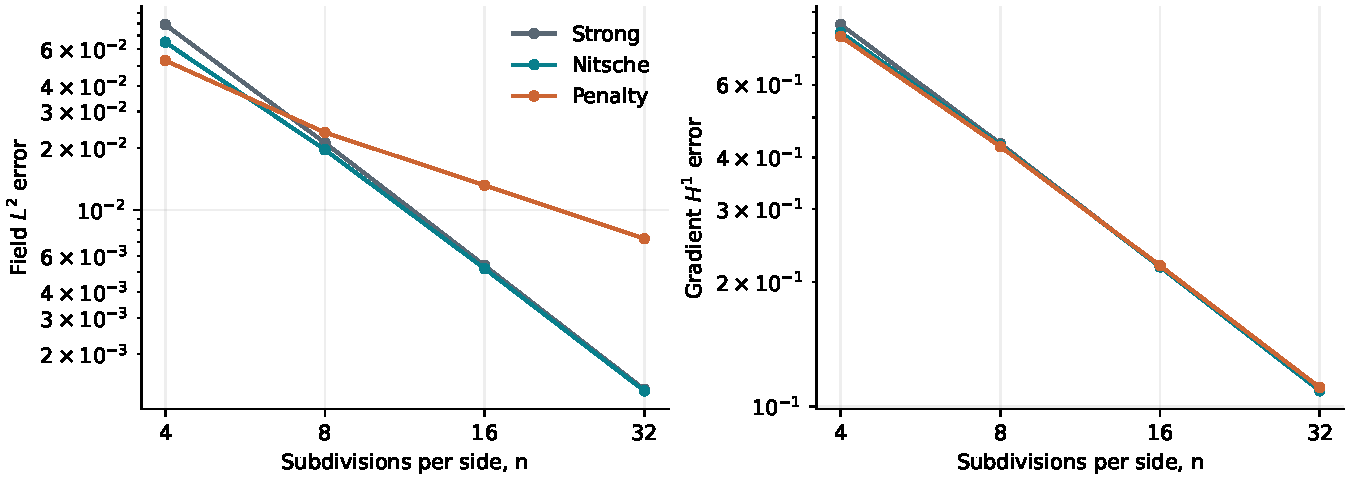
\includegraphics[width=\linewidth]{../examples/results/convergence.pdf}
\caption{Refinement at fixed $\gamma=10$. Strong and Nitsche results become
close with refinement. Penalty consistency bias impairs the field-error trend
even when gradient errors appear comparable. All curves are computed results.}
\label{fig:refine}
\end{figure}

\subsection{Quadrature and algebraic error are separate}
Increasing assembly quadrature from six to ten points per coordinate on $n=4$
changes the maximum load entry by $\QuadLoad$ and the computed Nitsche solution
by $\QuadSolve$. Raising error quadrature from eight to twelve changes the
largest reported norm by $\QuadNorm$.
At $n=8$, $\gamma=10$, Nitsche's scaled backward indicator is $\Residual$ while
its continuum $L^2$ error is $\CoarseL$. The indicator is
\begin{equation}
 \eta=\frac{\|A u_h-b\|_\infty}
 {\|A\|_\infty\|u_h\|_\infty+\|b\|_\infty}.
\end{equation}
For strong enforcement it uses the reduced equations. A small $\eta$ verifies
algebraic satisfaction; it neither estimates continuum error nor certifies
forward accuracy in a poorly conditioned system.

\newpage
\section{Parameter sensitivity and discussion}
At $n=8$ the condensed threshold is $\Critical$. Direct eigensolves at
$0.999\gamma_*$ and $1.001\gamma_*$ confirm a sign change of the smallest
full-matrix eigenvalue. The sweep excludes indefinite Nitsche matrices from
error and condition-number plots. Even the stable choice $\gamma=1.57$ gives
$L^2$ error $\NearL$ and matrix condition number $\NearCondition$; crossing
the threshold alone does not ensure useful accuracy.

\begin{figure}[h]
\centering
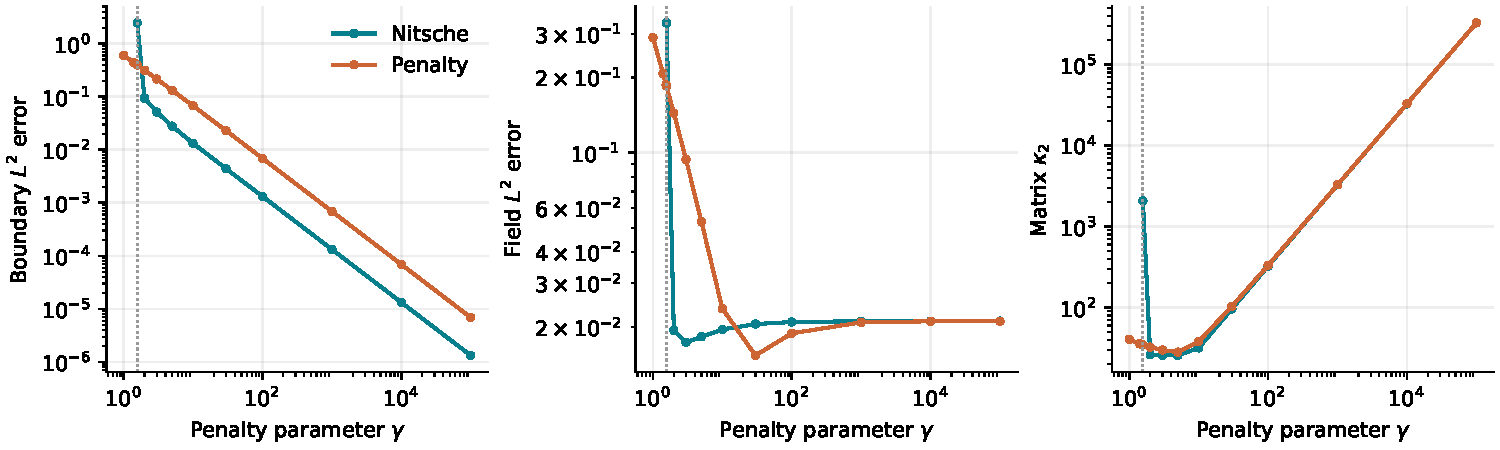
\includegraphics[width=\linewidth]{../examples/results/parameter.pdf}
\caption{Parameter study on $n=8$. Dotted lines mark $\gamma_*$. Only positive
definite cases are plotted; $\kappa_2$ is the ratio of extreme eigenvalues of
the unscaled full nodal matrix. The two methods approach strong enforcement
as $\gamma$ grows for this representable affine trace.}
\label{fig:parameter}
\end{figure}

Larger penalties suppress trace error, but the field error reaches a
discretization floor. At $\gamma=10^5$, Nitsche's condition number is
$\HighCondition$, without improved field accuracy. Penalty errors can also
partially cancel spatial errors on a coarse grid: one small total error does not
establish consistency or reliable convergence.

\section{Limitations and conclusion}
The Schur characterization holds in exact arithmetic; floating-point eigenvalues
are not interval bounds. Boundary-dense matrices limit scalability. Condition
numbers depend on basis scaling; no preconditioner is evaluated. Results concern
one smooth problem, one affine patch, uniform diagonal meshes and unit
coefficients. Singular solutions, distorted or cut elements, partial Dirichlet
boundaries and heterogeneous media require further analysis.

Boundary mismatch should be assessed alongside consistency and continuum error.
Nitsche recovers a linear patch and nearly second-order field convergence at a
moderate parameter; finite penalty retains boundary bias. Neither accurate
linear algebra nor manufactured-solution agreement establishes physical validity.
The repository contains original code, measured data, figures and build checks,
without course handouts, private datasets or experimental measurements.

\begin{thebibliography}{9}
\small
\bibitem{nitsche} J. Nitsche. \emph{\"Uber ein Variationsprinzip zur L\"osung
von Dirichlet-Problemen bei Verwendung von Teilr\"aumen, die keinen
Randbedingungen unterworfen sind}. Abh. Math. Sem. Univ. Hamburg 36,
9--15 (1971). \href{https://doi.org/10.1007/BF02995904}{doi:10.1007/BF02995904}.
\bibitem{dokken} J. S. Dokken. \emph{Weak imposition of Dirichlet conditions
for the Poisson problem}. FEniCSx tutorial.
\href{https://jsdokken.com/dolfinx-tutorial/chapter1/nitsche.html}{Public formulation and example}
(accessed 5 October 2026).
\bibitem{scipy} P. Virtanen et al. SciPy 1.0: fundamental algorithms for
scientific computing in Python. Nature Methods 17, 261--272 (2020).
\href{https://doi.org/10.1038/s41592-019-0686-2}{doi:10.1038/s41592-019-0686-2}.
\end{thebibliography}
\end{document}
